% ЕМТ 2025, X клас — точен LaTeX препис от официалните файлове в Klasirane.com.
% Условия: https://klasirane.com/api/competitions/EMT/All/2025/10%20%D0%BA%D0%BB/probs
% SHA-256 (условия): 09cd6962b96c019a5f90b943885c3f7237a372f68abd98f21b55fcf9472218a7
% Решения: https://klasirane.com/api/competitions/EMT/All/2025/10%20%D0%BA%D0%BB/sol
% SHA-256 (решения): 7a60daf2ef235abf307865b690dba6141d7c8cee1da28a7b77c545fca3ca0b54
% Точковите оценки, правописът и формулировките са запазени от източника.
% Файлът с условията е едностранично сканирано изображение; видимата страница е проверена пряко.
% Първата страница на файла с решенията съдържа и повторение на края на решение 9.4; то не е част от този препис.

Задача 10.1. Едно уравнение ще наричаме интересно, ако съществува реално число $c$, такова че за всеки реален корен на уравнението $x_0$ е в сила:

$$\sqrt{c+\frac{1}{x_0}}=\sqrt{c^2-x_0^2}.$$

а) Докажете, че уравнението $x^3-1=0$ е интересно.

б) Намерете за кои стойности на параметъра $a$ уравнението

$$x^4-x^3+ax^2+(1-a)x-1=0$$

има поне два реални корена и е интересно.

Решение. а) $x^3-1=0$ има единствен реален корен $x=1$. Значи за него трябва да е изпълнено условието: $c+1=c^2-1\Longrightarrow(c+1)(c-2)=0$, т.е. $c=2$ или $c=-1$. И за двете стойности на $c$ подкоренните величини са неотрицателни, така че уравнението със сигурност е интересно.

б) Разлагаме уравнението до следния вид: $(x-1)(x^3+ax+1)=0$. Отново имаме корен 1 и от а) следва, че $c\in\{2,-1\}$. Нека сега $x_0$ е корен на $x^3+ax+1=0$ (по условие, а и по принцип винаги съществува за уравнение от трета степен). Значи $x_0^3=-ax_0-1$. Използвайки равенството в условието, трябва да е в сила, че:

$$c+\frac{1}{x_0}=c^2-x_0^2\Longleftrightarrow\frac{x_0^3+1}{x_0}=c^2-c\Longleftrightarrow\frac{-ax_0-1+1}{x_0}=2\Longrightarrow a=-2.$$

Остава да проверим дали за всеки корен на уравнението $(x-1)(x^3-2x+1)=0$ подкоренните величини са неотрицателни. Имаме

$$(x-1)(x^3-2x+1)=0\Longleftrightarrow(x-1)^2(x^2+x-1)=0\Longleftrightarrow x\in\left\{1,\frac{-1\pm\sqrt5}{2}\right\}.$$

При $c=2$ това е изпълнено и следователно $a=-2$ е единствената стойност, за която даденото уравнение е интересно.

Оценяване. (6 точки) a) 1 т. за $c=2$ или $c=-1$; 1 т. за проверка на подкоренните величини; б) 1 т. за разлагането и $c\in\{2,-1\}$.; 1 т. за $a=-2$; 1 т. за пресмятане на корените; 1 т. за проверка на дефиниционната област.

Задача 10.2. Даден е триъгълник $ABC$ с описана окръжност $\omega$. Нека вътрешната и външната ъглополовяща на ъгъл $ACB$ пресичат правата $AB$ съответно в точки $D$ и $E$. Точки $I$ и $K$ лежат на правата $AC$ ($K$ е между $A$ и $I$) и са такива, че $DI=DC$ и $EC=EK$. Докажете, че правите $EK$ и $CD$ се пресичат върху $\omega$ тогава и само тогава, когато правите $EK$ и $DI$ се пресичат върху $\omega$.

Решение. Нека $DI\cap EK=P$, а $CD\cap EK=S$.

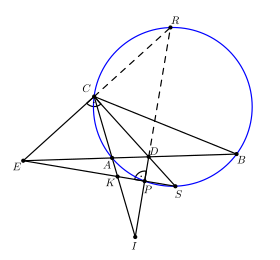
\includegraphics[max width=0.48\textwidth, alt={Официалната фигура към решение 10.2 с триъгълника ABC, окръжността и точките D, E, I, K, P, R и S}, center]{assets/10-2-geometry.svg}

(Първи начин) Нека допуснем, че $S\in\omega$. Тогава е в сила, че $SA=SB$. Пресмятаме $\angle EPD=\angle PKI+\angle PIK=\angle EKC+\angle DIC=\angle ECK+\angle DCI=90^\circ$ и следователно $DPEC$ е вписан четириъгълник, т.е. $SD.SC=SP.SE$. Но от $\triangle SAD\sim\triangle SCA$ знаем, че $SD.SC=SA^2=SB^2$. Следователно $SP.SE=SA^2=SB^2$, т.е. $\triangle SEA\sim\triangle SAP$ и $\triangle SEB\sim\triangle SBP$. Тогава $\angle SEA=\angle PAS$ и $\angle SEB=\angle PBS$. Но $\angle SEA=\angle SEB$, следователно $\angle PAS=\angle PBS$ и $P,S,B,A$ лежат на една окръжност, която е $\omega$.

Нека сега $P\in\omega$. Тогава $\angle DPC=\angle DEC=90^\circ-\frac12\gamma-\beta$, $\angle CPB=\angle CAB=\alpha$. Следователно $\angle BPS=\frac12\gamma=\angle BCS$ и $S\in\omega$.

(Втори начин) Нека $DI\cap EC=R$ и $\ell$ е допирателната към $\omega$ в точка $C$. Ще докажем, че описаните окръжности около $\triangle CRS$ и $\triangle ABC$ се допират вътрешно в точка $C$. От $DP\perp EP$ и $DC\perp EC$ следва, че $SRCP$ и $DPEC$ са вписани четириъгълници, т.е.

$$\angle CRS=\angle CPE=\angle CDE=\angle ABC+\angle BCD=\angle(\ell,AC)+\angle ACD=\angle(\ell,CD).$$

Но последното означава, че $\ell$ се допира и до описаната около $\triangle CRS$ окръжност $\omega'$. Следователно всяко едно от условията $S\in\omega$ или $P\in\omega$ е еквивалентно на $\omega\equiv\omega'$ и твърдението е доказано.

Оценяване. (6 точки) (Първи начин) $(\rightarrow)$ 1 т. за $DPEC$ вписан и $SP.SE=SD.SC$; 1 т. за $SD.SC=SA^2=SB^2$; 2 т. за $\angle PAS=\angle PEA=\angle PBS$ и $P\in\omega$; $(\leftarrow)$ 1 т. за $\angle BPS=\frac12\gamma$; 1 т. за $S\in\omega$. (Втори начин) 2 т. за построяването на точка $R$ и свеждане на задачата до доказване на факта, че описаната окръжност около $\triangle CRS$ се допира до $\omega$; 1 т. за $SRCP$ и $DPEC$ вписани; 3 т. за довършване.

Задача 10.3. В равнината са дадени 46 точки. Сумата от всевъзможните разстояния между тях е 2025. Да се докаже, че съществува затворена начупена линия, минаваща през всяка точка точно по веднъж, с дължина най-много 90.

Решение. (Първи начин) Ще докажем задачата в общ случай, а именно - ако имаме $N$ точки и сума $S$, не е възможно всяка затворена начупена линия да е с дължина повече от $\frac{2S}{N-1}$. Да допуснем, че е така.

Първо, броят на затворените начупени линии е $\frac{(N-1)!}{2}$, защото ако номерираме точките от 1 до $N$, всяка затворена линия е пермутация на тези числа. Тъй като е затворена, трябва да разделим на $N$ и тъй като имаме и две посоки на обхождане, делим и на 2. Значи сумата от всички начупени линии е повече от $\frac{(N-1)!}{2}.\frac{2S}{N-1}=S.(N-2)!$.

От друга страна, можем да преброим всяка отсечка в колко начупени затворени линии участва. Този брой е точно $(N-2)!$, което можем да обосновем по следния начин. Търсим броя на пермутациите, в които числата $a$ и $b$ са едно до друго. Този брой е $2.(N-1)!$. Сега делим отново на $2.(N-1)$ заради посоката и затвореността. Значи сумата от всички начупени линии е $S.(N-2)!$ - противоречие.

(Втори начин) Ще докажем с индукция по $N$, че при $N$ точки съществува Хамилтонов цикъл с дължина не повече от $2S_N/(N-1)$, където $S_N$ е сумата на всички разстояния между $N$-те точки. Базата на индукцията при $N=3$ е тривиална.

Да допуснем, че това е вярно за всеки $N-1$ точки, $N\ge4$. Да вземем произволни $N$ точки. Фиксираме една, да я кръстим $X_0$. За останалите $N-1$ точки прилагаме индукционното предположение. Т.е., съществува цикъл $X_1X_2\ldots X_{N-1}X_1$ с обща дължина $S'\le2S_{N-1}/(N-2)$, където $S_{N-1}$ е сумата от разстоянията м/у всеки две от точките $\{X_1,X_2,\ldots,X_{n-1}\}$. Да означим $\Delta S:=\sum_{i=1}^{n-1}X_0X_i$. Имаме

$$\min_i(X_0X_i+X_0X_{i+1}-X_iX_{i+1})\le\frac{1}{N-1}\left(2\sum_{i=1}^{N-1}X_0X_i-S'\right)=\frac{2\Delta S}{N-1}-\frac{S'}{N-1}.$$

Следователно

$$\begin{aligned}
\min_i(X_0X_{i+1}X_{i+2}\ldots X_iX_0)
&=\min_i(X_0X_i+X_0X_{i+1}-X_iX_{i+1})+S'\\
&\le\frac{2\Delta S}{N-1}-\frac{S'}{N-1}+S'=\frac{2\Delta S}{N-1}+\frac{N-2}{N-1}S'\\
&\le\frac{2\Delta S}{N-1}+\frac{N-2}{N-1}\cdot\frac{2S_{N-1}}{N-2}=\frac{2\Delta S+2S_{N-1}}{N-1}\\
&=\frac{2S_N}{N-1}.
\end{aligned}$$

Оценяване. (7 точки) 1 т. за правилно обобщение на твърдението. В случай, че това се прави последно или не се прави, точката се прехвърля при довършване; 1 т. за разглеждане на подход със сумиране; 2 т. за преброяване на броя на затворените начупени линии с обосновка (обосновката е 1 точка); 2 т. за преброяване на броя срещания на всяка отсечка с обосновка; 1 т. за довършване.

Задача 10.4. Дадени са две ненулеви цели числа $m$ и $n$, които са взаимно прости. Да се намерят всички функции $f:\mathbb Z\to\mathbb Z$, такива че:

$$f(m.x+n.y)=mf(f(x))+nf(f(y))$$

Решение. (Първи начин) Нека положим $g(x)=f(f(x))$. Тогава

$$f(mx)=mg(x)+ng(0)\tag{1}$$

От друга страна $mx=m(x+nt)-nmt$ и можем да заместим. Получаваме, че за всяко $t$ и всяко $x$:

$$f(mx)=mg(x+nt)+ng(-mt)\tag{2}$$

Приравнявайки (1) и (2) и замествайки $t=1$, получаваме:

$$mg(x+n)+ng(-m)=mg(x)+ng(0)\Longleftrightarrow g(x+n)-g(x)=\frac{n}{m}(g(0)-g(-m))\tag{3}$$

Дясната страна не зависи от $x$, значи получаваме, че $g(x+n)-g(x)=C_1$. Аналогично получаваме, че $g(x+m)-g(x)=C_2$. Но $g(mn)=g(0)+mC_1=g(0)+nC_2$, откъдето $C_2=\frac{m}{n}C_1$. Сега, от Безу следва, че има числа $p,q$, такива че $1=mp+nq$. Получаваме следната връзка:

$$g(x+1)=g(x+mp+nq)=g(x+mp)+qC_1=g(x)+pC_2+qC_1.$$

Значи $g(x)$ е линейна функция. т.е. $f(f(x))=ax+b$. Връщаме се в условието на задачата: $f(mx+ny)=m(ax+b)+n(ay+b)=a(mx+ny)+b(m+n)$. Но всяко едно число може да се представи във вида $z=mx+by$, така че $f(z)=az+b(m+n)$ за всяко $z$.

Значи, замествайки във $f(f(x))=ax+b$, получаваме, че $f(ax+b(m+n))=a^2x+ab(m+n)+b(m+n)\Longrightarrow a^2x+ab(m+n)+bm+bn=ax+b$.

Tъй като това е равенство за всяко $x$, имаме, че $a^2=a$ и $ab(m+n)+b(m+n)=b$. Имаме два случая: $a=0$ или $a=1$:

• $a=0\Longrightarrow b(m+n)=b$. Ако $m+n=1$, тогава $f(x)\equiv C$, а ако не, то $f(x)\equiv0$.

• $a=1\Longrightarrow2b(m+n)=b$. Следователно $b=0$ и $f(x)=x$.

Отговор: Ако $m+n=1$, то $f(x)=C$ или $f(x)=x$; Ако $m+n\neq1$, то $f(x)=0$ или $f(x)=x$;

(Втори начин) Последователно имаме, че

1. $P(x,y)=(x,0)\Longrightarrow f(mx)=mf(f(x))+nf(f(0))$

2. $P(x,y)=(0,x)\Longrightarrow f(nx)=nf(f(x))+mf(f(0))$

3. $P(0,0)\Longrightarrow f(0)=(m+n)f(f(0))$

4. $f(mx+ny)=f(mx)+f(ny)-f(0)$

От последното с индукция $x$ следва, че

$$f(mnx)=x\big(f(mn)-f(0)\big)+f(0)\quad\forall x\in\mathbb Z$$

Да отбележим също, че $1.\Longrightarrow f(mx)\equiv nf(f(0))\equiv(m+n)f(f(0))\equiv f(0)\pmod m$ и $2.\Longrightarrow f(nx)\equiv f(0)\pmod n$, т.е $f(mn)\equiv f(0)\pmod{mn}$, т.е $f(mn)-f(0)=mna$ за някое $a\in\mathbb Z$, т.к $(m,n)=1$.

Така получаваме, че $(5)$ $f(mnx)=amnx+f(0)$ за $x\in\mathbb Z$.

От (1), (3) и (5) имаме, че

$$\begin{aligned}
amnx+f(0)&=f(mnx)=mf(f(nx))+nf(f(0))\\
amnx&=mf(f(nx))-mf(f(0))\\
f(f(nx))&=anx+f(f(0))
\end{aligned}$$

и аналогично

$$f(f(mx))=amx+f(f(0)).$$

Сега замествайки в (1) получаваме

$$amx+f(f(0))=f(f(mx))=f(mf(f(x))+nf(f(0)))=mf^{(4)}(x)+nf^{(4)}(0)$$

$$f^{(4)}(x)=ax+b,$$

където $b=(f(f(0))-nf^{(4)}(0))/m$. Сега, замествайки в равенството от условието получаваме

$$\begin{aligned}
f(f(mx+ny))&=f(mf(f(x))+nf(f(y)))=mf^{(4)}(x)+nf^{(4)}(y)\\
&=a(mx+ny)+b(m+n)
\end{aligned}$$

От Безу, т.к $(m,n)=1$ получаваме, че $f(f(x))=ax+b$ за $x\in\mathbb Z$ и решението се довършва, както горното с директна проверка.

Оценяване. (7 точки) 5 т. за линейност на $f(f(x))$, от които 2 т. за подходящи субституции, водещи към прогрес като (1) и (2) в първото решение и (1), (2), (3) и (4) във второто решение; 2 т. за довършване, ако $f(f(x))$ е линейна, като 1 т. се дава за изчерпателен отговор.
